% Provenance (never printed): cycle 4 SVT, "La planete Terre, l'environnement
% et l'action humaine": the relief as a balance between uplift and erosion;
% landforms of the wind, the sea and dissolution; reading a landscape; see
% sources/book1/PROVENANCE.md. Book 1, grade 9, chapter 4.
% Vocabulary guard: owns uplift, dune, cliff, beach and spit (with longshore
% drift), karst (with cave and sinkhole). Landscape and landform are g1's;
% weathering, erosion, deposition, meander and delta are g5's; relief is
% g4's; plates and mountain building are g7's; U-shaped valley and moraine
% are g8's; limestone and the acid test are g6's; acids are the chemistry
% books' (recalled in prose). Contour lines are g9.5's (not used here).
% "Normal fault" and the destruction of mountains are Book 2's.
\chapter{Landvormen}\label{ch:g9:landforms}

Aan de zuidkust van Engeland vallen de witte \omterm{def:g9:landforms:cliff}{kliffen} van de Seven Sisters
loodrecht in \omterm{def:g2:water-on-earth:ocean}{zee}. In een gewoon jaar verliezen ze tot een meter. In de
winter van 2014 namen \omterm{def:g5:natural-hazards:storm}{stormen} in twee maanden evenveel weg van de \omterm{def:g9:landforms:cliff}{kliffen}
bij Birling Gap als ze gewoonlijk in zeven jaar verliezen. Het krijt van
deze \omterm{def:g9:landforms:cliff}{kliffen} was ooit modder op de bodem van een \omterm{def:g2:water-on-earth:ocean}{zee}, opgebouwd uit de
piepkleine plaatjes van microscopische algen die in het water leefden. Nu
staat het er als een muur van wit \omterm{def:g3:stones-pebbles-sand:rock}{gesteente}, die de golven elk jaar weer
een stukje verder terugdringen. Waarom heeft het land de vormen die het
heeft, en waarom veranderen sommige daarvan zo snel?
% ledger: nt:birling-2014, sdnp:birling, nasa:coccoliths

\begin{omfigure}
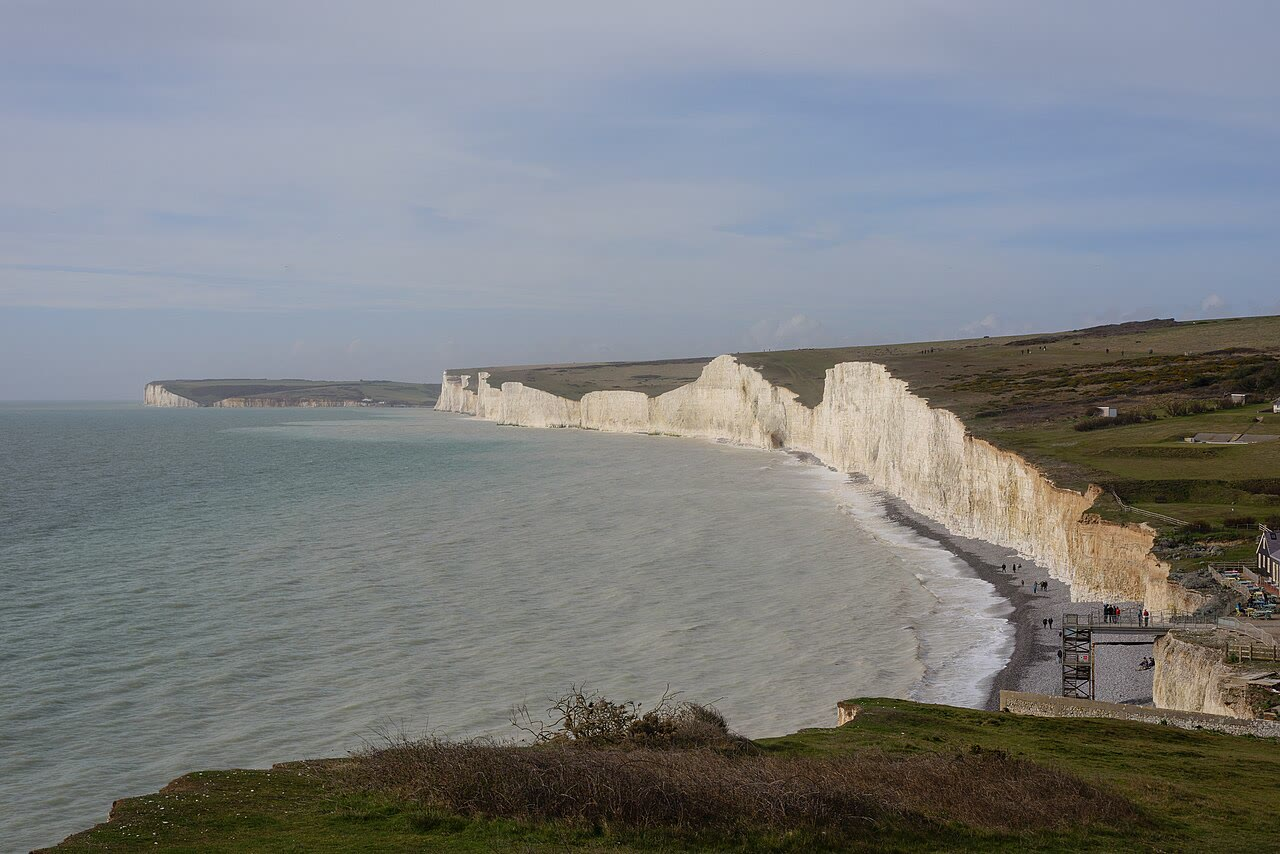
\includegraphics[width=\linewidth]{images/book1/g9-seven-sisters.jpg}

{\small De Seven Sisters, krijtkliffen aan de \omterm{def:g1:landscapes-around-us:water}{kust} van East Sussex
(Engeland), met op de voorgrond de huizen van Birling Gap. De \omterm{def:g2:water-on-earth:ocean}{zee} drijft de
\omterm{def:g9:landforms:cliff}{kliffen} terug, en op elk moment kan er \omterm{def:g3:stones-pebbles-sand:rock}{gesteente} naar beneden storten. Aan
hun voet ligt een kiezelstrand. Foto van Arild Vågen, 2017 (CC BY-SA 4.0,
via Wikimedia Commons).}
% ledger: commons:seven-sisters, sdnp:birling
\label{fig:g9:landforms:seven-sisters}
\end{omfigure}

\begin{recall}
Een \emph{\omterm{def:g1:landscapes-around-us:landform}{landvorm}} is één vorm van het land: een \omterm{def:g1:landscapes-around-us:landform}{heuvel}, een \omterm{def:g1:landscapes-around-us:landform}{dal}, een
\omterm{def:g1:landscapes-around-us:landform}{vlakte}, een \omterm{def:g9:landforms:cliff}{klif} (\cref{ch:g1:landscapes-around-us}). Het \omterm{def:g4:world-physical-map:relief}{reliëf} is de vorm
van het land in de hoogte (\cref{ch:g4:world-physical-map}). \omterm{def:g5:water-shapes-the-land:weathering}{Verwering}
breekt het \omterm{def:g3:stones-pebbles-sand:rock}{gesteente}, \omterm{def:g5:water-shapes-the-land:erosion}{erosie} slijt het af en voert het weg, en \omterm{def:g5:water-shapes-the-land:deposition}{afzetting}
legt het elders neer (\cref{ch:g5:water-shapes-the-land}). De \omterm{def:g7:plate-tectonics:plate}{platen} duwen
\omterm{def:g4:world-physical-map:range}{gebergten} omhoog waar ze botsen (\cref{ch:g7:plate-tectonics}); \omterm{def:g8:ice-on-earth:glacier}{gletsjers}
slijten \omterm{def:g8:ice-on-earth:glacial-landforms}{U-dalen} uit (\cref{ch:g8:ice-on-earth}); kalksteen bruist onder een
druppel verdund zuur (\cref{ch:g6:rocks-and-minerals}). In de scheikunde
leer je dat zuren kalksteen aantasten en daarbij kooldioxide vrijmaken.
\end{recall}

\section{Het reliëf: een evenwicht tussen opheffing en erosie}

Twee soorten krachten vormen het \omterm{def:g4:world-physical-map:relief}{reliëf}. Van binnenuit heffen de
bewegingen van de \omterm{def:g7:plate-tectonics:plate}{platen} de grond op. Van buitenaf slijten water, ijs, wind
en de \omterm{def:g2:water-on-earth:ocean}{zee} hem weer af.

\begin{definition}[Opheffing]\label{def:g9:landforms:uplift}
\emph{Opheffing}\index{opheffing} is het langzame omhoogkomen van het
\omterm{def:g3:stones-pebbles-sand:rock}{gesteente} en het grondoppervlak van een gebied, aangedreven door krachten
in het binnenste van de Aarde, zoals de botsing van twee \omterm{def:g7:plate-tectonics:plate}{platen}.
\end{definition}

\omterm{def:g9:landforms:uplift}{Opheffing} is traag op de schaal van een mensenleven, maar snel op de schaal
van de Aarde. India botste ongeveer 50~miljoen jaar geleden met Azië, en
het Tibetaans Plateau, achter de Himalaya, kreeg het grootste deel van zijn
hoogte, ongeveer \qty{4600}{m}, in de laatste 10~miljoen jaar. Gemiddeld is
dat $4600 \div 10^7 = 4.6 \times 10^{-4}$~m, of ongeveer \qty{0.5}{mm} per
jaar: minder dan de dikte van een vingernagel, maar miljoenen jaren lang
volgehouden.
% ledger: usgs:himalaya (rate computed in figdata/grade-9/cliff_retreat.py, tibet_rate_mm_yr)

Zodra de grond stijgt, valt de \omterm{def:g5:water-shapes-the-land:erosion}{erosie} hem aan. Hoe hoger en steiler het
land, hoe sneller \omterm{def:g1:landscapes-around-us:water}{rivieren}, \omterm{def:g8:ice-on-earth:glacier}{gletsjers} en vallend \omterm{def:g3:stones-pebbles-sand:rock}{gesteente} het materiaal
afvoeren. De hoogte van een \omterm{def:g4:world-physical-map:range}{gebergte} is op elk moment de uitkomst van een
wedstrijd: wat de \omterm{def:g9:landforms:uplift}{opheffing} omhoogbrengt, min wat de \omterm{def:g5:water-shapes-the-land:erosion}{erosie} wegneemt.

\begin{omfigure}
\begin{tikzpicture}[font=\footnotesize, >={Stealth[length=2mm]}]
  % panel 1: uplift faster than erosion
  \begin{scope}
    \fill[black!13] (0,0) -- (0.5,0) .. controls (1.1,1.0) and (1.5,2.0) .. (1.8,2.2)
      .. controls (2.1,2.0) and (2.5,1.0) .. (3.1,0) -- (3.6,0) -- (3.6,-0.5) -- (0,-0.5) -- cycle;
    \draw[black!60] (0,0) -- (0.5,0) .. controls (1.1,1.0) and (1.5,2.0) .. (1.8,2.2)
      .. controls (2.1,2.0) and (2.5,1.0) .. (3.1,0) -- (3.6,0);
    \draw[black!60, dashed] (0.7,0) .. controls (1.2,0.8) and (1.5,1.5) .. (1.8,1.6)
      .. controls (2.1,1.5) and (2.4,0.8) .. (2.9,0);
    \foreach \x in {1.2,1.8,2.4} \draw[->, omWarm, line width=1.4pt] (\x,-0.45) -- ++(0,1.0);
    \draw[->, omRiver, thick] (2.15,1.6) -- ++(0.35,-0.3);
    \node[align=center, anchor=north] at (1.8,-0.6) {opheffing sneller\\dan erosie:\\het reliëf stijgt};
  \end{scope}
  % panel 2: uplift equals erosion
  \begin{scope}[xshift=4.4cm]
    \fill[black!13] (0,0) -- (0.5,0) .. controls (1.1,1.0) and (1.5,1.8) .. (1.8,1.9)
      .. controls (2.1,1.8) and (2.5,1.0) .. (3.1,0) -- (3.6,0) -- (3.6,-0.5) -- (0,-0.5) -- cycle;
    \draw[black!60] (0,0) -- (0.5,0) .. controls (1.1,1.0) and (1.5,1.8) .. (1.8,1.9)
      .. controls (2.1,1.8) and (2.5,1.0) .. (3.1,0) -- (3.6,0);
    \foreach \x in {1.2,1.8,2.4} \draw[->, omWarm, line width=1.4pt] (\x,-0.45) -- ++(0,0.6);
    \draw[->, omRiver, thick] (2.05,1.6) -- ++(0.55,-0.5);
    \draw[->, omRiver, thick] (1.55,1.6) -- ++(-0.55,-0.5);
    \node[align=center, anchor=north] at (1.8,-0.6) {opheffing en erosie\\even sterk: de\\hoogte blijft gelijk};
  \end{scope}
  % panel 3: no more uplift
  \begin{scope}[xshift=8.8cm]
    \fill[black!13] (0,0) -- (0.4,0) .. controls (1.1,0.5) and (1.5,0.95) .. (1.8,1.0)
      .. controls (2.1,0.95) and (2.5,0.5) .. (3.2,0) -- (3.6,0) -- (3.6,-0.5) -- (0,-0.5) -- cycle;
    \draw[black!60] (0,0) -- (0.4,0) .. controls (1.1,0.5) and (1.5,0.95) .. (1.8,1.0)
      .. controls (2.1,0.95) and (2.5,0.5) .. (3.2,0) -- (3.6,0);
    \draw[black!60, dashed] (0.5,0) .. controls (1.1,1.0) and (1.5,1.8) .. (1.8,1.9)
      .. controls (2.1,1.8) and (2.5,1.0) .. (3.1,0);
    \draw[->, omRiver, thick] (2.05,0.95) -- ++(0.55,-0.5);
    \draw[->, omRiver, thick] (1.55,0.95) -- ++(-0.55,-0.5);
    \node[align=center, anchor=north] at (1.8,-0.6) {geen opheffing meer:\\de erosie verlaagt\\het reliëf};
  \end{scope}
  % key
  \draw[->, omWarm, line width=1.4pt] (13.2,1.2) -- ++(0,0.6) node[right, black] {opheffing};
  \draw[->, omRiver, thick] (13.2,0.7) -- ++(0.35,-0.3) node[right, black] {erosie};
  \draw[black!60, dashed] (13.1,-0.1) -- ++(0.5,0) node[right, black] {vroeger profiel};
\end{tikzpicture}

{\small Het \omterm{def:g4:world-physical-map:relief}{reliëf} als evenwicht (een schets, niet op schaal). \omterm{def:g9:landforms:uplift}{Opheffing}
tilt het \omterm{def:g3:stones-pebbles-sand:rock}{gesteente} op; \omterm{def:g5:water-shapes-the-land:erosion}{erosie} voert het af naar de \omterm{def:g1:landscapes-around-us:landform}{dalen} en de \omterm{def:g2:water-on-earth:ocean}{zee}. Een
\omterm{def:g4:world-physical-map:range}{gebergte} blijft groeien zolang de \omterm{def:g9:landforms:uplift}{opheffing} wint; als de \omterm{def:g7:plate-tectonics:plate}{platen} niet meer
duwen, slijt de \omterm{def:g5:water-shapes-the-land:erosion}{erosie} het langzaam af tot \omterm{def:g1:landscapes-around-us:landform}{heuvels}.}
\label{fig:g9:landforms:balance}
\end{omfigure}

\omterm{def:g1:landscapes-around-us:water}{Rivieren} (\cref{ch:g5:water-shapes-the-land}) en \omterm{def:g8:ice-on-earth:glacier}{gletsjers}
(\cref{ch:g8:ice-on-earth}) zijn de grote beeldhouwers van \omterm{def:g4:world-physical-map:range}{gebergten}. De
rest van dit hoofdstuk volgt drie andere krachten, die elk hun eigen
\omterm{def:g1:landscapes-around-us:landform}{landvormen} maken: de wind, de \omterm{def:g2:water-on-earth:ocean}{zee}, en water dat \omterm{def:g3:stones-pebbles-sand:rock}{gesteente} oplost.

\section{Landvormen van de wind: duinen}

Waar weinig planten groeien, veel los \omterm{def:g3:stones-pebbles-sand:sand}{zand} ligt en de wind sterk is, kan de
wind \omterm{def:g3:stones-pebbles-sand:sand}{zand} opnemen en het tot \omterm{def:g1:landscapes-around-us:landform}{heuvels} ophopen: in \omterm{def:g5:weather-and-climate:desert}{woestijnen}, en achter
zandstranden.
% ledger: nps:aeolian

\begin{definition}[Duin]\label{def:g9:landforms:dune}
Een \emph{duin}\index{duin} is een hoop of een rug van los \omterm{def:g3:stones-pebbles-sand:sand}{zand}, door de
wind opgehoopt. De helling die naar de wind gekeerd is, is lang en flauw;
de andere kant, de \emph{lijzijde}\index{lijzijde}, is kort en steil.
\end{definition}
% ledger: nps:aeolian, nmt:barchan

Een \omterm{def:g9:landforms:dune}{duin} beweegt. De wind laat de korrels rollend en springend de flauwe
helling op gaan; op de kam hopen ze zich op tot de hoop te steil wordt, en
een kleine lawine van \omterm{def:g3:stones-pebbles-sand:sand}{zand} glijdt langs de \omterm{def:g9:landforms:dune}{lijzijde} naar beneden. Korrel na
korrel wordt \omterm{def:g3:stones-pebbles-sand:sand}{zand} van de loefzijde weggenomen en aan de andere kant
neergelegd, en het hele \omterm{def:g9:landforms:dune}{duin} kruipt met de wind mee zonder ooit te worden
opgetild. \omterm{def:g9:landforms:dune}{Duinen} staan zelden alleen: ze vormen hele duinvelden.
% ledger: nmt:barchan, nps:aeolian

Waar de wind altijd uit dezelfde richting waait en het \omterm{def:g3:stones-pebbles-sand:sand}{zand} niet al te
overvloedig is, krijgen \omterm{def:g9:landforms:dune}{duinen} de vorm van een sikkel, een
\emph{barchaan}: de ronde neus is naar de wind gekeerd en de twee hoorns
wijzen met de wind mee. De hoorns bevatten minder \omterm{def:g3:stones-pebbles-sand:sand}{zand} dan het midden, dus
bewegen ze sneller en strekken ze zich voor het \omterm{def:g9:landforms:dune}{duin} uit.
% ledger: nmt:barchan

\begin{omfigure}
\begin{tikzpicture}[font=\footnotesize, >={Stealth[length=2mm]}]
  % plan view
  \fill[yellow!25!orange!20] (3.4,1.3) .. controls (1.0,1.3) and (0.2,0.6) .. (0.2,0)
     .. controls (0.2,-0.6) and (1.0,-1.3) .. (3.4,-1.3)
     .. controls (2.4,-0.9) and (1.8,-0.5) .. (1.8,0)
     .. controls (1.8,0.5) and (2.4,0.9) .. (3.4,1.3) -- cycle;
  \fill[orange!45] (3.4,1.3) .. controls (2.4,0.9) and (1.8,0.5) .. (1.8,0)
     .. controls (1.8,-0.5) and (2.4,-0.9) .. (3.4,-1.3)
     .. controls (2.1,-0.8) and (1.45,-0.45) .. (1.45,0)
     .. controls (1.45,0.45) and (2.1,0.8) .. (3.4,1.3) -- cycle;
  \draw[black!60] (3.4,1.3) .. controls (1.0,1.3) and (0.2,0.6) .. (0.2,0)
     .. controls (0.2,-0.6) and (1.0,-1.3) .. (3.4,-1.3)
     .. controls (2.4,-0.9) and (1.8,-0.5) .. (1.8,0)
     .. controls (1.8,0.5) and (2.4,0.9) .. (3.4,1.3);
  \draw[black, thick] (3.4,1.3) .. controls (2.1,0.8) and (1.45,0.45) .. (1.45,0)
     .. controls (1.45,-0.45) and (2.1,-0.8) .. (3.4,-1.3);
  \foreach \y in {-0.8,0,0.8} \draw[->, omRiver, thick] (-1.3,\y) -- ++(1.1,0);
  \node[above] at (-0.75,0.85) {wind};
  \node[anchor=west] at (3.5,1.35) {hoorn};
  \node[anchor=west] at (3.5,-1.35) {hoorn};
  \draw[black!70] (1.75,0.25) -- (2.9,0.35) node[anchor=west, align=left, black] {lijzijde\\(steil)};
  \draw[black!70] (0.75,-0.2) -- (0.6,-1.6) node[anchor=north, align=center, black] {loefzijde\\(flauw)};
  \draw[black!70] (1.47,-0.3) -- (2.4,-1.75) node[anchor=north, black] {kam};
  \node[anchor=south, font=\footnotesize\bfseries] at (1.4,1.6) {van boven gezien};
  % profile
  \begin{scope}[xshift=7.2cm, yshift=-0.8cm]
    \draw[black!60] (-0.4,0) -- (5.6,0);
    \fill[yellow!25!orange!20] (0,0) -- (3.0,1.2) -- (3.6,0) -- cycle;
    \draw[black!70] (0,0) -- (3.0,1.2) -- (3.6,0);
    \fill[orange!45] (3.0,1.2) -- (3.6,0) -- (3.3,0) -- cycle;
    \draw[black!50, dashed] (0.8,0) -- (3.8,1.2) -- (4.4,0);
    \draw[->, black!70] (0.5,0.35) .. controls (0.75,0.65) .. (1.0,0.45);
    \draw[->, black!70] (1.0,0.55) .. controls (1.25,0.85) .. (1.5,0.65);
    \draw[->, black!70] (1.5,0.75) .. controls (1.75,1.05) .. (2.0,0.85);
    \draw[->, black!70] (2.0,0.95) .. controls (2.25,1.25) .. (2.5,1.05);
    \draw[->, thick, black!80] (3.15,1.05) -- (3.45,0.35);
    \foreach \y in {1.6,2.1} \draw[->, omRiver, thick] (-0.8,\y) -- ++(1.1,0);
    \node[above] at (-0.25,2.1) {wind};
    \draw[->, thick] (4.5,0.6) -- ++(0.7,0) node[right, align=left] {het duin\\beweegt};
    \node[align=center, anchor=north] at (1.2,-0.1) {korrels springen\\de flauwe helling op};
    \node[align=center, anchor=north west] at (2.9,-0.1) {en glijden langs\\de lijzijde af};
    \node[anchor=south, font=\footnotesize\bfseries] at (2.2,2.3) {van opzij gezien};
  \end{scope}
\end{tikzpicture}

{\small Een sikkelduin, of barchaan (een schets). Van boven gezien wijzen
de hoorns met de wind mee. Van opzij gezien klimmen de korrels de flauwe
loefzijde op en glijden ze langs de steile \omterm{def:g9:landforms:dune}{lijzijde} naar beneden: het \omterm{def:g9:landforms:dune}{duin}
beweegt met de wind mee (stippellijn: het \omterm{def:g9:landforms:dune}{duin} even later).}
% ledger: nmt:barchan, nps:aeolian
\label{fig:g9:landforms:barchan}
\end{omfigure}

Hoe snel? In het gipsduinveld van White Sands, in New Mexico, bewegen de
kleine \omterm{def:g9:landforms:dune}{duinen} die aan de rand aan de windkant ontstaan, een paar meter
hoog, tot \qty{6}{m} per jaar; iets verderop, als ze 6 tot \qty{10}{m} hoog
zijn geworden, bewegen ze ongeveer \qty{3}{m} per jaar. Hoe meer \omterm{def:g3:stones-pebbles-sand:sand}{zand} een
\omterm{def:g9:landforms:dune}{duin} bevat, hoe trager het gaat. Barchanen die door sterke winden worden
voortgedreven, kunnen meer dan \qty{100}{m} per jaar afleggen, genoeg om een
weg of een akker te begraven.
% ledger: nps:whsa-migration, nmt:barchan

\begin{omfigure}
\begin{minipage}[c]{0.5\linewidth}\centering
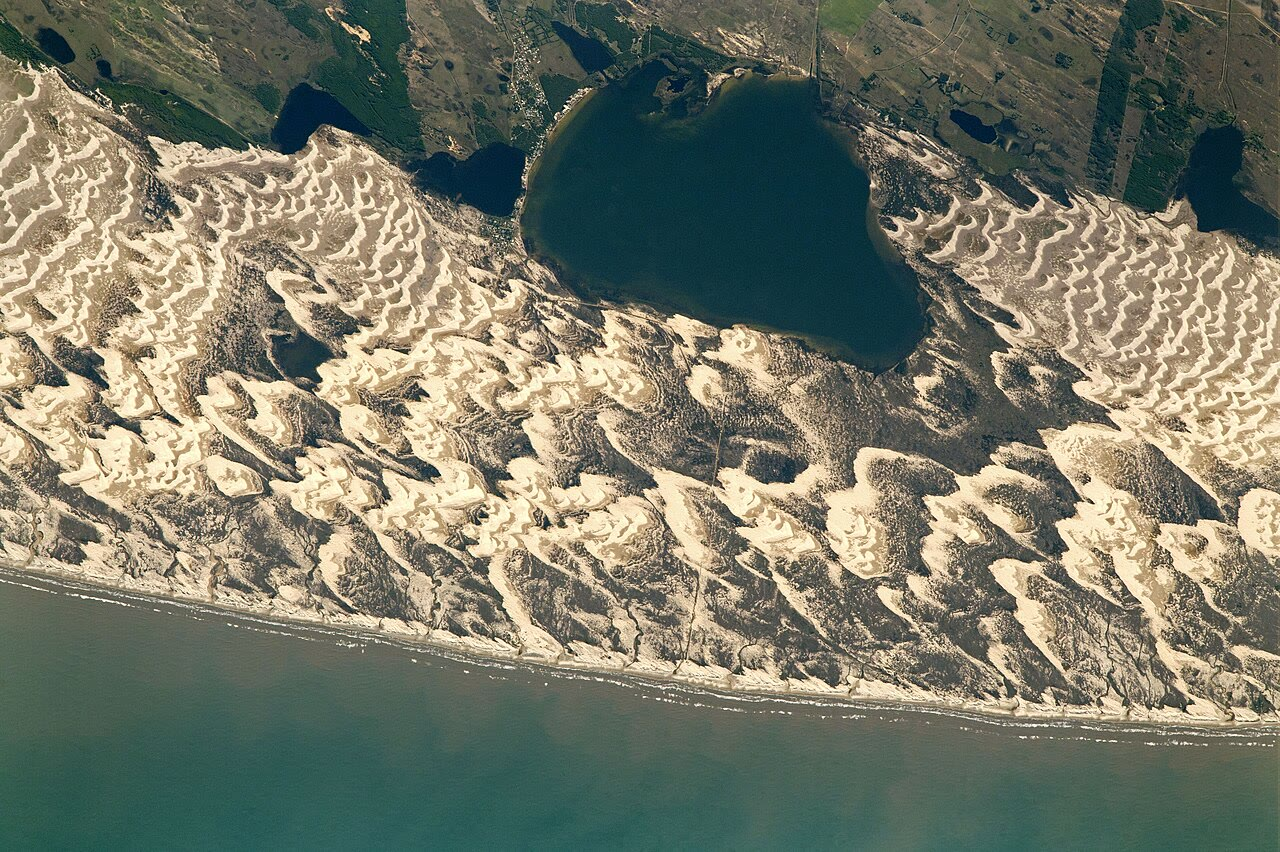
\includegraphics[width=\linewidth]{images/book1/g9-barchans.jpg}
\end{minipage}\hfill
\begin{minipage}[c]{0.46\linewidth}\raggedright
{\small Sikkelvormige \omterm{def:g9:landforms:dune}{duinen} aan de Atlantische \omterm{def:g1:landscapes-around-us:water}{kust} van Zuid-Brazilië, in
2017 gefotografeerd door een astronaut vanuit het Internationaal
Ruimtestation. Het donkere meer, Lagoa dos Barros, is ongeveer
\qty{4.5}{km} lang. Het \omterm{def:g3:stones-pebbles-sand:sand}{zand} komt van het \omterm{def:g9:landforms:beach}{strand}, onder aan de foto. NASA
(publiek domein, via Wikimedia Commons).}
\end{minipage}
% ledger: commons:iss-barchans
\label{fig:g9:landforms:barchans-photo}
\end{omfigure}

Aan een \omterm{def:g1:landscapes-around-us:water}{kust} beschermt een rij \omterm{def:g9:landforms:dune}{duinen} achter het \omterm{def:g9:landforms:beach}{strand} het land daarachter
tegen stormgolven. Planten die op de \omterm{def:g9:landforms:dune}{duinen} groeien, houden het \omterm{def:g3:stones-pebbles-sand:sand}{zand} met
hun wortels vast: waar ze worden vertrapt of weggehaald, neemt de wind het
\omterm{def:g3:stones-pebbles-sand:sand}{zand} weer mee.
% ledger: nps:aeolian

\section{Landvormen van de zee}

\subsection{Kliffen}

\begin{definition}[Klif]\label{def:g9:landforms:cliff}
Een \emph{klif}\index{klif} is een steile of loodrechte rotswand. Aan een
\omterm{def:g1:landscapes-around-us:water}{kust} wordt een klif door de golven uitgesleten: ze vallen de voet ervan aan
en laten het landinwaarts terugwijken.
\end{definition}

De golven slingeren water, \omterm{def:g3:stones-pebbles-sand:sand}{zand} en \omterm{def:g3:stones-pebbles-sand:pebble}{kiezels} tegen de voet van het \omterm{def:g9:landforms:cliff}{klif}.
Beetje bij beetje slijten ze aan de basis een holte uit, een
\emph{inkeping}, tussen het niveau van eb en dat van vloed. Het \omterm{def:g3:stones-pebbles-sand:rock}{gesteente}
erboven hangt over; \omterm{def:g4:clouds-rain-snow:precipitation}{regen} en vorst verzwakken het verder. Op een dag stort
de overhang in. De golven breken de gevallen blokken en voeren ze weg, en
de aanval begint opnieuw op een verse wand, iets verder landinwaarts. Het
terugwijkende \omterm{def:g9:landforms:cliff}{klif} laat een vlakke rotsbank achter, het
\emph{abrasieplatform}\index{abrasieplatform}, dat bij eb droogvalt.
% ledger: nt:birling-2014, sdnp:birling

Zacht \omterm{def:g3:stones-pebbles-sand:rock}{gesteente} wijkt het snelst terug. Bij Birling Gap verliezen de
krijtkliffen tot ongeveer een meter per jaar; maar het terugwijken gaat met
sprongen, één instorting tegelijk, en een stormachtige winter kan in één
keer jaren van terugwijken meenemen. In 1999 werd de oude vuurtoren Belle
Tout, in 1832 gebouwd boven op de \omterm{def:g9:landforms:cliff}{kliffen} in de buurt, in één stuk
\qty{17}{m} van de rand af verplaatst, omdat het \omterm{def:g9:landforms:cliff}{klif} te dichtbij kwam.
% ledger: sdnp:birling, nt:birling-2014

\begin{omfigure}
\begin{tikzpicture}[font=\footnotesize, >={Stealth[length=2mm]}]
  % panel 1: the notch
  \begin{scope}
    \fill[omSea!45] (0,-0.1) rectangle (1.8,0.75);
    \fill[omSea!45] (1.8,0.35) -- (2.25,0.55) -- (1.8,0.95) -- cycle;
    \fill[black!8] (1.6,-0.1) -- (1.8,0.25) -- (1.8,0.35) -- (2.25,0.55) -- (1.8,0.95) -- (1.8,2.4) -- (3.6,2.4) -- (3.6,-0.6) -- (0,-0.6) -- (0,-0.1) -- cycle;
    \draw[black!70] (0,-0.1) -- (1.6,-0.1) -- (1.8,0.25) -- (1.8,0.35) -- (2.25,0.55) -- (1.8,0.95) -- (1.8,2.4) -- (3.6,2.4);
    \foreach \y in {0.8,1.3,1.8} \draw[black!25] (1.8,\y) -- (3.6,\y);
    \fill[green!35!black!50] (1.8,2.4) rectangle (3.6,2.5);
    \draw[->, omSea!80!black, thick] (0.4,0.6) -- (1.6,0.6);
    \node[anchor=south, align=center] at (0.9,0.8) {golven};
    \draw[black!70] (2.15,0.55) -- (2.9,1.0) node[anchor=west, fill=white, inner sep=1pt] {inkeping};
    \node[anchor=north, align=center] at (1.8,-0.7) {1. de golven slijten\\een inkeping uit};
    \node[anchor=south, font=\footnotesize] at (2.7,2.5) {krijt};
  \end{scope}
  % panel 2: collapse
  \begin{scope}[xshift=4.6cm]
    \fill[omSea!45] (0,-0.1) rectangle (2.2,0.75);
    \fill[black!8] (2.0,-0.1) -- (2.2,0.25) -- (2.25,2.4) -- (3.6,2.4) -- (3.6,-0.6) -- (0,-0.6) -- (0,-0.1) -- cycle;
    \draw[black!70] (0,-0.1) -- (2.0,-0.1) -- (2.2,0.25) -- (2.25,2.4) -- (3.6,2.4);
    \draw[black!50, dashed] (1.8,0.95) -- (1.8,2.4) -- (2.25,2.4);
    \foreach \y in {0.8,1.3,1.8} \draw[black!25] (2.25,\y) -- (3.6,\y);
    \fill[green!35!black!50] (2.25,2.4) rectangle (3.6,2.5);
    \foreach \x/\y/\s in {1.25/0.05/0.28, 1.6/0.1/0.22, 1.95/0.3/0.3, 1.45/0.35/0.18}
      \fill[black!20, draw=black!60] (\x,\y) rectangle ++(\s,\s*0.8);
    \node[anchor=north, align=center] at (1.8,-0.7) {2. de overhang\\stort in};
  \end{scope}
  % panel 3: retreat and platform
  \begin{scope}[xshift=9.2cm]
    \fill[omSea!45] (0,0.2) rectangle (2.8,0.75);
    \fill[black!8] (0,0.0) -- (2.6,0.2) -- (2.8,0.3) -- (2.85,2.4) -- (4.0,2.4) -- (4.0,-0.6) -- (0,-0.6) -- cycle;
    \draw[black!70] (0,0.0) -- (2.6,0.2) -- (2.8,0.3) -- (2.85,2.4) -- (4.0,2.4);
    \foreach \y in {0.8,1.3,1.8} \draw[black!25] (2.85,\y) -- (4.0,\y);
    \fill[green!35!black!50] (2.85,2.4) rectangle (4.0,2.5);
    \draw[black!50, dashed] (1.4,0.12) -- (1.4,2.4);
    \draw[black!50, dashed] (2.1,0.16) -- (2.1,2.4);
    \draw[<-, thick] (2.8,1.6) -- (1.5,1.6);
    \node[anchor=south, align=center] at (1.4,2.45) {vroegere klifwanden};
    \node[anchor=north, align=center] at (2.0,-0.7) {3. een abrasieplatform,\\droog bij eb};
  \end{scope}
\end{tikzpicture}

{\small Hoe een zeeklif terugwijkt (een schets, niet op schaal). (1) De
golven slijten een inkeping uit aan de voet van het \omterm{def:g9:landforms:cliff}{klif}. (2) Het
overhangende \omterm{def:g3:stones-pebbles-sand:rock}{gesteente} stort in; de golven breken de blokken en voeren ze
weg. (3) De cyclus herhaalt zich: het \omterm{def:g9:landforms:cliff}{klif} schuift landinwaarts op en laat
een vlak rotsplatform voor zich achter.}
% ledger: nt:birling-2014, sdnp:birling
\label{fig:g9:landforms:cliff-retreat}
\end{omfigure}

\begin{safety}
De rand van een \omterm{def:g9:landforms:cliff}{klif} kan op elk moment afbrokkelen, en er vallen zonder
waarschuwing stenen van de wand. \omterm{def:g9:landforms:cliff}{Kliffen} bekijk je van een veilige afstand,
boven ver van de rand en op het \omterm{def:g9:landforms:beach}{strand} ver van de voet, en een \omterm{def:g9:landforms:beach}{strand} onder
\omterm{def:g9:landforms:cliff}{kliffen} verlaat je voordat de vloed opkomt.
\end{safety}
% ledger: nt:birling-2014, sdnp:birling

\subsection{Stranden en landtongen}

Het \omterm{def:g3:stones-pebbles-sand:sand}{zand} en de \omterm{def:g3:stones-pebbles-sand:pebble}{kiezels} die van \omterm{def:g9:landforms:cliff}{kliffen} afslijten, en die \omterm{def:g1:landscapes-around-us:water}{rivieren} aanvoeren,
blijven niet liggen waar ze vallen: de golven sorteren ze en verplaatsen ze
langs de \omterm{def:g1:landscapes-around-us:water}{kust}.

\begin{definition}[Strand, kustlangstransport en landtong]\label{def:g9:landforms:beach}
Een \emph{strand}\index{strand} is een strook \omterm{def:g3:stones-pebbles-sand:sand}{zand} of \omterm{def:g3:stones-pebbles-sand:pebble}{kiezels} die de golven
langs de oever hebben opgehoopt. Als de golven schuin op de \omterm{def:g1:landscapes-around-us:water}{kust} aankomen,
duwt elke golf de korrels onder die hoek het strand op en loopt het water
recht langs de helling terug: de korrels zigzaggen langs de \omterm{def:g1:landscapes-around-us:water}{kust}. Deze
verplaatsing van \omterm{def:g3:stones-pebbles-sand:sand}{zand} en \omterm{def:g3:stones-pebbles-sand:pebble}{kiezels} langs de oever is het
\emph{kustlangstransport}\index{kustlangstransport}. Een
\emph{landtong}\index{landtong} is een lange, smalle rug van \omterm{def:g3:stones-pebbles-sand:sand}{zand} of \omterm{def:g3:stones-pebbles-sand:pebble}{kiezels}
die door kustlangstransport is opgebouwd, aan één kant met het land
verbonden en uitlopend in \omterm{def:g2:water-on-earth:ocean}{zee} waar de \omterm{def:g1:landscapes-around-us:water}{kust} een bocht maakt.
\end{definition}
% ledger: noaa:longshore

Waar de \omterm{def:g1:landscapes-around-us:water}{kust} buigt, bij de monding van een baai of een \omterm{def:g1:landscapes-around-us:water}{rivier}, gaat het
transport in dezelfde richting door en laat het zijn lading vallen in het
rustigere water: het \omterm{def:g9:landforms:beach}{strand} groeit als een \omterm{def:g9:landforms:beach}{landtong} de \omterm{def:g2:water-on-earth:ocean}{zee} in. Het uiteinde
krult vaak naar binnen, omgebogen door golven uit andere richtingen. Achter
de \omterm{def:g9:landforms:beach}{landtong}, beschut tegen de golven, bezinkt modder en groeien kwelders.
% ledger: noaa:longshore

\begin{omfigure}
\begin{tikzpicture}[font=\footnotesize, >={Stealth[length=2mm]}]
  % sea
  \fill[omSea!40] (0,0) rectangle (11,2.3);
  % land with a bay
  \fill[green!25!black!20] (0,2.3) -- (6,2.3) .. controls (6.3,3.0) and (7.0,3.5) .. (8.0,3.5)
     .. controls (9.0,3.5) and (9.3,2.8) .. (9.5,2.3) -- (11,2.3) -- (11,4.6) -- (0,4.6) -- cycle;
  % calm water of the bay
  \fill[omSea!20] (6,2.3) .. controls (6.3,3.0) and (7.0,3.5) .. (8.0,3.5)
     .. controls (9.0,3.5) and (9.3,2.8) .. (9.5,2.3) -- cycle;
  % salt marsh
  \fill[green!50!black!35] (6.15,2.55) .. controls (6.6,3.1) and (7.3,3.2) .. (7.9,3.0)
     .. controls (7.6,2.7) and (7.0,2.6) .. (6.15,2.55) -- cycle;
  \node[anchor=west, font=\scriptsize] at (6.5,3.85) {kwelder};
  \draw[black!60] (6.9,3.75) -- (7.0,2.95);
  % river
  \draw[omRiver, line width=1.2pt] (8.6,4.6) .. controls (8.5,4.0) and (8.3,3.7) .. (8.3,3.48);
  \node[anchor=west, font=\scriptsize] at (8.65,4.25) {rivier};
  % beach
  \fill[yellow!40!orange!35] (0,1.85) rectangle (6,2.3);
  % spit
  \fill[yellow!40!orange!35] (5.9,1.85) .. controls (7.0,1.95) and (7.8,2.0) .. (8.35,2.1)
     .. controls (8.6,2.2) and (8.6,2.5) .. (8.4,2.65) -- (8.25,2.55)
     .. controls (8.35,2.45) and (8.3,2.35) .. (8.15,2.32)
     .. controls (7.5,2.28) and (6.8,2.3) .. (6.0,2.3) -- cycle;
  \draw[black!60] (0,2.3) -- (6,2.3) .. controls (6.3,3.0) and (7.0,3.5) .. (8.0,3.5)
     .. controls (9.0,3.5) and (9.3,2.8) .. (9.5,2.3) -- (11,2.3);
  % waves arriving at an angle
  \foreach \x in {0.9,2.0,3.1,4.2} \draw[omSea!70!black, line width=0.5pt] (\x,1.15) -- ++(-35:1.1);
  \draw[->, omSea!70!black, thick] (0.6,0.3) -- ++(55:1.2) node[pos=0.15, left, black] {golven};
  % zigzag of a pebble
  \draw[->, black, thick] (1.0,1.9) -- (1.35,2.2) -- (1.35,1.9) -- (1.7,2.2) -- (1.7,1.9)
     -- (2.05,2.2) -- (2.05,1.9) -- (2.4,2.2) -- (2.4,1.9);
  \node[anchor=south, align=center, font=\scriptsize] at (1.7,2.45) {schuin het strand\\op, recht weer\\naar beneden};
  % drift arrow
  \draw[->, line width=1.6pt, omWarm] (3.0,1.55) -- (5.6,1.55) node[midway, below, black] {kustlangstransport};
  % spit label
  \draw[black!70] (7.4,2.05) -- (7.6,1.2) node[anchor=north, align=center, black] {de landtong groeit\\dwars over de baai};
  \draw[->, thick, omWarm] (8.6,1.95) -- ++(0.6,0);
  % compass
  \draw[->] (10.4,0.3) -- ++(0,0.6) node[above] {N};
\end{tikzpicture}

{\small \omterm{def:g9:landforms:beach}{Kustlangstransport} en een \omterm{def:g9:landforms:beach}{landtong}, van boven gezien (een schets).
De golven komen uit het zuidwesten; elke golf duwt het \omterm{def:g3:stones-pebbles-sand:sand}{zand} en de \omterm{def:g3:stones-pebbles-sand:pebble}{kiezels}
schuin het \omterm{def:g9:landforms:beach}{strand} op, en het water loopt recht terug naar beneden: de
korrels zigzaggen naar het oosten. Waar de \omterm{def:g1:landscapes-around-us:water}{kust} een baai vormt, gaat het
transport door en bouwt het een \omterm{def:g9:landforms:beach}{landtong}, waarachter een kwelder groeit.
De \omterm{def:g1:landscapes-around-us:water}{rivier} houdt aan het uiteinde van de \omterm{def:g9:landforms:beach}{landtong} een geul open.}
% ledger: noaa:longshore
\label{fig:g9:landforms:spit}
\end{omfigure}

\begin{omfigure}
\begin{minipage}[c]{0.5\linewidth}\centering
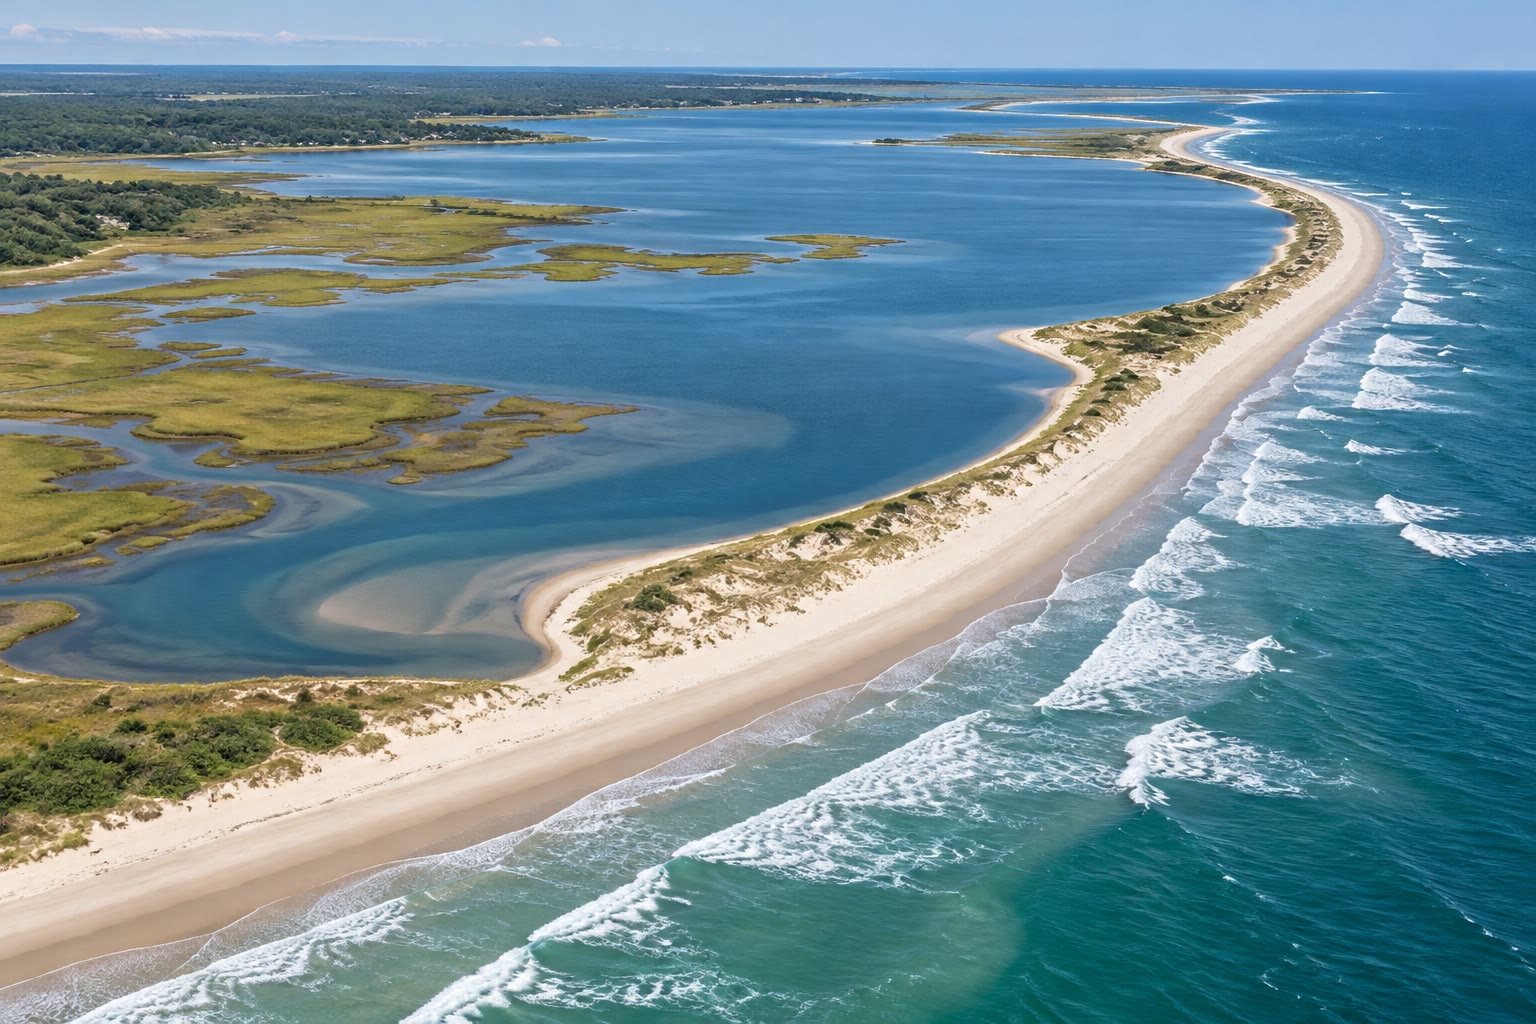
\includegraphics[width=\linewidth]{images/book1/ai/g9-spit-aerial.jpg}
\end{minipage}\hfill
\begin{minipage}[c]{0.46\linewidth}\raggedright
{\small Een zandige \omterm{def:g9:landforms:beach}{landtong} dwars over de monding van een baai, gezien
vanuit een laagvliegend vliegtuig (een illustratie, geen bestaande plek).
De golven breken op het \omterm{def:g9:landforms:beach}{strand} aan de zeekant; erachter liggen rustig water
en kwelders.}
\end{minipage}
\label{fig:g9:landforms:spit-ai}
\end{omfigure}

\section{Landvormen door oplossing: karst}

Regenwater is geen zuiver water. Als het door de lucht valt en daarna door
de bodem sijpelt, neemt het kooldioxide op, waardoor het licht zuur wordt.
Dit zwakke zuur doet langzaam wat de druppel verdund zuur snel doet met een
stukje kalksteen: het lost het \omterm{def:g3:stones-pebbles-sand:rock}{gesteente} op. Kalksteen zit vol spleten,
langs de lagen en dwars erdoor. Water sijpelt erdoorheen naar beneden en
verwijdt ze, millimeter voor millimeter, in duizenden jaren.
% ledger: usgs:sinkholes, nps:karst

\begin{definition}[Karst, grot en zinkgat]\label{def:g9:landforms:karst}
\emph{Karst}\index{karst} is een \omterm{def:g1:landscapes-around-us:landscape}{landschap} dat is gevormd door water dat
een oplosbaar \omterm{def:g3:stones-pebbles-sand:rock}{gesteente} oplost, meestal kalksteen. \omterm{def:g1:landscapes-around-us:water}{Rivieren} verdwijnen er
vaak onder de grond en komen verderop als bronnen weer tevoorschijn. Een
\emph{grot}\index{grot} is een natuurlijke ondergrondse ruimte die groot
genoeg is om er als mens in te gaan, ontstaan doordat het \omterm{def:g3:stones-pebbles-sand:rock}{gesteente} langs
zijn spleten is opgelost. Een \emph{zinkgat}\index{zinkgat} is een kuil of
een gat in het aardoppervlak, ontstaan waar het \omterm{def:g3:stones-pebbles-sand:rock}{gesteente} eronder wegoplost
of waar het dak van een grot instort.
\end{definition}
% ledger: nps:karst, usgs:sinkholes

\begin{omfigure}
\begin{tikzpicture}[x=0.9cm, y=0.9cm, font=\footnotesize, >={Stealth[length=2mm]}]
  \pic (B) at (0,0) {blockdiagram={10}{4}{4}};
  % top face: grassland
  \fill[green!25!black!18] (B-ftl) -- (B-ftr) -- (B-btr) -- (B-btl) -- cycle;
  % right face
  \fill[omLithLime!70] (B-fbr) -- (B-bbr) -- (B-btr) -- (B-ftr) -- cycle;
  % front face: limestone layers
  \fill[omLithLime] (B-fbl) rectangle (B-ftr);
  \foreach \y in {0.8,1.6,2.4,3.2} \draw[black!35] (0,\y) -- (10,\y);
  \foreach \x/\y in {1.2/0.8, 3.1/1.6, 4.6/0, 6.8/2.4, 8.3/0.8, 2.2/2.4, 9.1/2.4, 5.6/3.2}
    \draw[black!35] (\x,\y) -- ++(0,0.8);
  % soil
  \fill[brown!45] (0,3.8) rectangle (10,4);
  % sinkhole on the top face and in the front face
  \fill[green!25!black!35] (3.0,4.45) ellipse (0.7 and 0.22);
  \fill[white] (2.3,4) -- (3.7,4) -- (3.25,3.45) -- (2.75,3.45) -- cycle;
  \fill[green!25!black!30] (2.3,4) -- (3.7,4) -- (3.25,3.45) -- (2.75,3.45) -- cycle;
  \draw[black!60] (2.3,4) -- (2.75,3.45) -- (3.25,3.45) -- (3.7,4);
  % shaft from sinkhole to cave
  \fill[white] (2.85,3.45) -- (3.15,3.45) -- (3.35,2.0) -- (3.05,2.0) -- cycle;
  \draw[black!60] (2.85,3.45) -- (3.05,2.0) (3.15,3.45) -- (3.35,2.0);
  % cave
  \fill[white] (2.6,2.1) .. controls (3.5,2.35) and (5.5,2.3) .. (6.6,1.9)
     .. controls (7.4,1.6) and (7.6,1.2) .. (7.2,1.0)
     .. controls (6.0,0.85) and (4.0,1.0) .. (3.0,1.2)
     .. controls (2.3,1.35) and (2.1,1.9) .. (2.6,2.1) -- cycle;
  \draw[black!70] (2.6,2.1) .. controls (3.5,2.35) and (5.5,2.3) .. (6.6,1.9)
     .. controls (7.4,1.6) and (7.6,1.2) .. (7.2,1.0)
     .. controls (6.0,0.85) and (4.0,1.0) .. (3.0,1.2)
     .. controls (2.3,1.35) and (2.1,1.9) .. (2.6,2.1);
  % underground stream at the cave floor
  \fill[omRiver!60] (3.0,1.2) .. controls (4.0,1.0) and (6.0,0.85) .. (7.2,1.0) -- (7.1,1.12)
     .. controls (6.0,1.0) and (4.0,1.12) .. (3.1,1.3) -- cycle;
  % stalactites and stalagmites
  \foreach \x/\l in {4.2/0.35, 4.5/0.22, 4.9/0.4, 5.3/0.25, 5.8/0.3}
    \fill[black!45] (\x-0.07,2.22) -- (\x+0.06,2.22) -- (\x,2.22-\l) -- cycle;
  \foreach \x/\l in {4.9/0.3, 5.8/0.25}
    \fill[black!45] (\x-0.12,0.95) -- (\x+0.12,0.95) -- (\x,0.95+\l) -- cycle;
  % disappearing stream on the top face
  \draw[omRiver, line width=1.2pt] (7.4,4.85) .. controls (6.9,4.5) and (6.4,4.4) .. (6.0,4.25);
  \fill[black!70] (6.0,4.25) circle (0.07);
  \draw[omRiver, dashed, thick] (6.0,4.0) -- (6.4,2.1);
  % spring on the right face
  \draw[omRiver, line width=1.2pt, ->] (10.2,1.2) .. controls (10.8,1.1) and (11.2,0.7) .. (11.6,0.5);
  % rain with carbon dioxide
  \foreach \x in {0.6,1.2,1.8} \draw[->, omRiver] (\x,5.6) -- ++(-0.15,-0.7);
  \draw[->, omRiver, dashed] (1.0,3.9) -- (1.2,1.7);
  % outline
  \draw[black!70] (B-fbl) rectangle (B-ftr);
  \draw[black!70] (B-ftl) -- (B-btl) -- (B-btr) -- (B-ftr) (B-btr) -- (B-bbr) -- (B-fbr);
  % labels
  \node[anchor=south, align=center] at (1.2,5.6) {regen neemt kooldioxide\\op: licht zuur};
  \node[anchor=east, align=right] at (-0.1,1.6) {water verwijdt\\de spleten};
  \draw[black!70] (-0.05,1.6) -- (1.1,2.0);
  \node[anchor=south] at (3.0,5.2) {zinkgat};
  \draw[black!70] (3.0,5.2) -- (3.0,4.55);
  \node[anchor=south, align=center] at (7.6,5.3) {een beek verdwijnt\\onder de grond};
  \draw[black!70] (7.0,5.3) -- (6.1,4.35);
  \node[anchor=north, align=center] at (5.0,-0.1) {een grot: stalactieten hangen aan het plafond,\\stalagmieten groeien op uit de bodem};
  \draw[black!70] (5.0,-0.1) -- (5.0,1.4);
  \node[anchor=west, align=left] at (11.6,0.6) {bron};
  \node[anchor=west] at (11.9,3.4) {kalksteen};
\end{tikzpicture}

{\small Een karstlandschap (een schets, niet op schaal). Licht zuur water
sijpelt door de spleten van de kalksteen en verwijdt ze; ondergrondse beken
hollen \omterm{def:g9:landforms:karst}{grotten} uit; een grotdak bezwijkt en opent een \omterm{def:g9:landforms:karst}{zinkgat}; een beek
verdwijnt in een gat en komt lager als \omterm{def:g6:water-underground:spring}{bron} weer tevoorschijn.}
% ledger: nps:karst, usgs:sinkholes, nps:speleothems
\label{fig:g9:landforms:karst}
\end{omfigure}

In een \omterm{def:g9:landforms:karst}{grot} kan het oplossen omgekeerd verlopen. Een druppel water die uit
het dak sijpelt, bevat opgeloste kalksteen. Als hij de lucht van de \omterm{def:g9:landforms:karst}{grot}
raakt, staat hij een deel van zijn kooldioxide af, en rond de druppel slaat
een dun laagje calciet uit het water neer. Druppel na druppel groeit er een
holle buis uit het dak, die daarna dikker wordt tot een
\emph{stalactiet}\index{stalactiet}, die als een ijspegel naar beneden
hangt. Waar de druppels neerkomen, bouwt de rest van het calciet een
\emph{stalagmiet}\index{stalagmiet} op vanaf de bodem. Als de twee elkaar
raken, vormen ze een zuil.
% ledger: nps:speleothems

\begin{omfigure}
\begin{minipage}[c]{0.5\linewidth}\centering
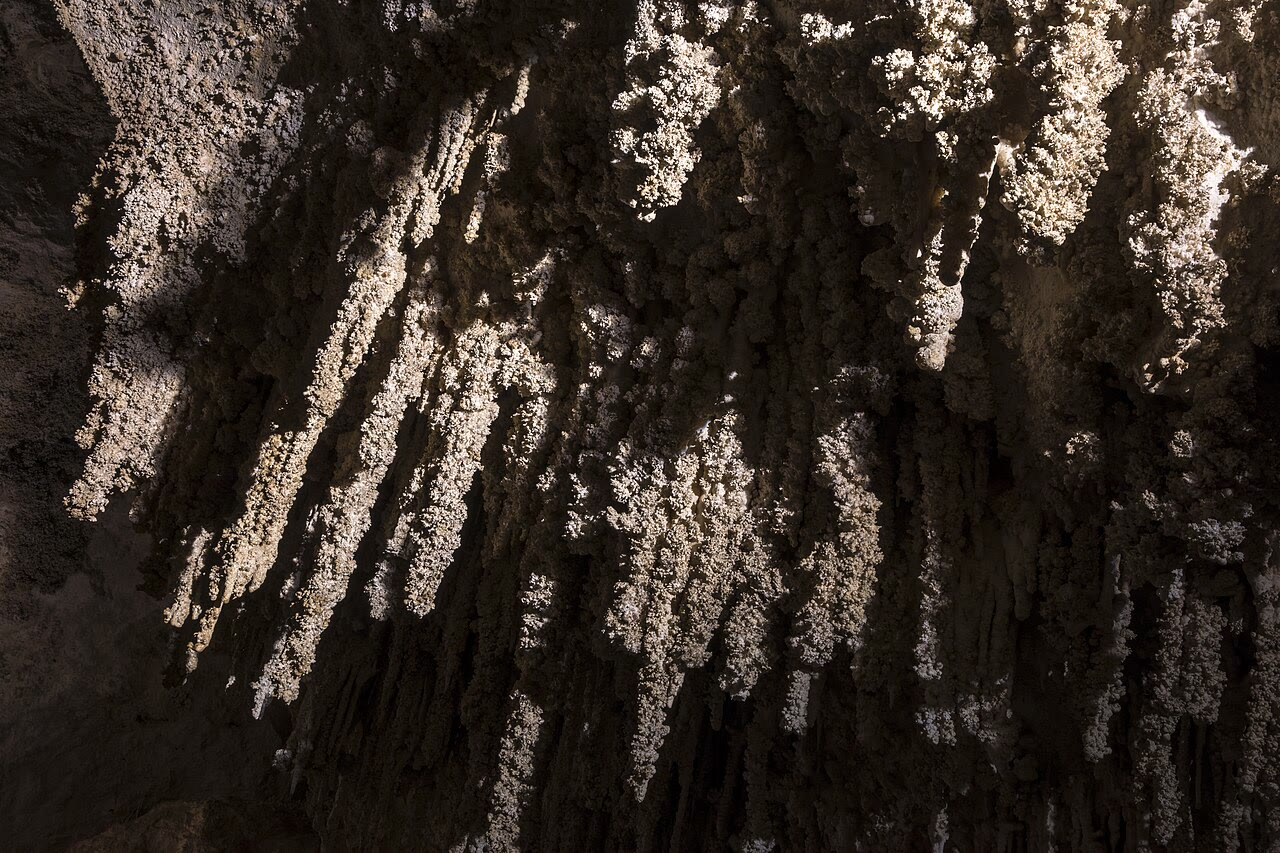
\includegraphics[width=\linewidth]{images/book1/g9-stalactites.jpg}
\end{minipage}\hfill
\begin{minipage}[c]{0.46\linewidth}\raggedright
{\small Stalactieten die onder een groot rotsblok hangen in Carlsbad
Cavern, New Mexico, een \omterm{def:g9:landforms:karst}{grot} die in kalksteen is uitgelost. Elke
stalactiet groeide druppel voor druppel uit water dat door het \omterm{def:g3:stones-pebbles-sand:rock}{gesteente}
erboven sijpelde. National Park Service, 2018 (publiek domein, via
Wikimedia Commons).}
\end{minipage}
% ledger: commons:carlsbad-stalactites, nps:speleothems
\label{fig:g9:landforms:stalactites}
\end{omfigure}

Een karstgebied bevat veel water onder de grond, maar dat stroomt snel door
de open spleten en wordt nauwelijks gefilterd: wat op de grond wordt
gemorst, kan snel een \omterm{def:g6:water-underground:spring}{bron} bereiken. En waar het \omterm{def:g3:stones-pebbles-sand:rock}{gesteente} eronder is
opgelost, kan de grond inzakken of instorten: waar mensen wonen, kan een
\omterm{def:g9:landforms:karst}{zinkgat} dat plotseling opengaat wegen en huizen verzwelgen.
% ledger: nps:karst, usgs:sinkholes

\section{Een landschap lezen}

Elke \omterm{def:g1:landscapes-around-us:landform}{landvorm} is een aanwijzing. Zijn vorm vertelt welke kracht hem heeft
gemaakt; de kracht vertelt welk proces aan het werk was, \omterm{def:g5:water-shapes-the-land:erosion}{erosie} of
\omterm{def:g5:water-shapes-the-land:deposition}{afzetting}; en het proces zegt vaak iets over het \omterm{def:g3:stones-pebbles-sand:rock}{gesteente} of het losse
materiaal eronder.

\begin{method}[Een landvorm lezen]
\begin{enumerate}
  \item \textbf{Vorm.} Beschrijf de \omterm{def:g1:landscapes-around-us:landform}{landvorm}: een rug, een kuil, een steile
        wand, een vlakke bank; zijn grootte; naar welke kant hij wijst.
  \item \textbf{Kracht en proces.} Bepaal welke kracht hem heeft gemaakt
        (een \omterm{def:g1:landscapes-around-us:water}{rivier}, ijs, de wind, de \omterm{def:g2:water-on-earth:ocean}{zee}, oplossend water) en of hij is
        uitgesleten (\omterm{def:g5:water-shapes-the-land:erosion}{erosie}) of opgebouwd (\omterm{def:g5:water-shapes-the-land:deposition}{afzetting}).
  \item \textbf{Materiaal.} Zeg waarvan hij is gemaakt, of wat het \omterm{def:g3:stones-pebbles-sand:rock}{gesteente}
        eronder waarschijnlijk is: los \omterm{def:g3:stones-pebbles-sand:sand}{zand}, \omterm{def:g3:stones-pebbles-sand:pebble}{kiezels}, kalksteen, hard of
        zacht \omterm{def:g3:stones-pebbles-sand:rock}{gesteente}.
\end{enumerate}
\end{method}

\begin{center}
{\small
\begin{tabular}{|>{\raggedright\arraybackslash}p{4.6cm}|>{\raggedright\arraybackslash}p{2.6cm}|>{\raggedright\arraybackslash}p{2.2cm}|>{\raggedright\arraybackslash}p{2.6cm}|}
\hline
vorm & kracht & proces & materiaal \\
\hline
sikkelvormige zandheuvels & wind & \omterm{def:g5:water-shapes-the-land:deposition}{afzetting} & los \omterm{def:g3:stones-pebbles-sand:sand}{zand} \\
een loodrechte rotswand boven een vlakke rotsbank & \omterm{def:g2:water-on-earth:ocean}{zee} & \omterm{def:g5:water-shapes-the-land:erosion}{erosie} & \omterm{def:g3:stones-pebbles-sand:rock}{gesteente} (zacht \omterm{def:g3:stones-pebbles-sand:rock}{gesteente} wijkt snel terug) \\
een smalle zandrug dwars over een baai & \omterm{def:g2:water-on-earth:ocean}{zee} (transport langs de \omterm{def:g1:landscapes-around-us:water}{kust}) & \omterm{def:g5:water-shapes-the-land:deposition}{afzetting} & \omterm{def:g3:stones-pebbles-sand:sand}{zand} of \omterm{def:g3:stones-pebbles-sand:pebble}{kiezels} \\
kuilen in akkers, beken die verdwijnen & oplossend water & oplossing & kalksteen \\
een \omterm{def:g8:ice-on-earth:glacial-landforms}{U-dal} & ijs & \omterm{def:g5:water-shapes-the-land:erosion}{erosie} & elk \omterm{def:g3:stones-pebbles-sand:rock}{gesteente} \\
een waaier van modder bij een riviermonding & \omterm{def:g1:landscapes-around-us:water}{rivier} & \omterm{def:g5:water-shapes-the-land:deposition}{afzetting} & modder en \omterm{def:g3:stones-pebbles-sand:sand}{zand} \\
\hline
\end{tabular}}
\end{center}

\begin{example}[Een wandeling op een plateau]
Op een hoog, grazig plateau is helemaal geen beek, hoewel het er vaak
regent. De velden zijn bezaaid met ronde kuilen van een paar meter breed,
en in het \omterm{def:g1:landscapes-around-us:landform}{dal} eronder spuit een krachtige \omterm{def:g6:water-underground:spring}{bron} uit de voet van een
rotswand. \emph{Vorm}: kuilen, geen beken aan het oppervlak, een \omterm{def:g6:water-underground:spring}{bron}
lager. \emph{Kracht en proces}: water dat het \omterm{def:g3:stones-pebbles-sand:rock}{gesteente} oplost en onder de
grond stroomt. \emph{Materiaal}: het plateau bestaat hoogstwaarschijnlijk
uit kalksteen, en de kuilen zijn \omterm{def:g9:landforms:karst}{zinkgaten}. Een druppel verdund zuur op een
los stukje van het \omterm{def:g3:stones-pebbles-sand:rock}{gesteente}, aangebracht door de leraar, zou bruisen.
\end{example}
% ledger: nps:karst, usgs:sinkholes

\section{Oefeningen}

\begin{exercise}[$\star$]\label{exo:g9:landforms:1}
Welke kracht heeft elke \omterm{def:g1:landscapes-around-us:landform}{landvorm} gemaakt: de wind, de \omterm{def:g2:water-on-earth:ocean}{zee}, een \omterm{def:g1:landscapes-around-us:water}{rivier}, ijs,
of water dat het \omterm{def:g3:stones-pebbles-sand:rock}{gesteente} oplost? (a) Een sikkelvormige zandheuvel in een
\omterm{def:g5:weather-and-climate:desert}{woestijn}. (b) Een \omterm{def:g9:landforms:karst}{grot} vol stalactieten. (c) Een lange kiezelrug dwars over
de monding van een baai. (d) Een \omterm{def:g8:ice-on-earth:glacial-landforms}{U-dal} met een \omterm{def:g8:ice-on-earth:glacial-landforms}{morene} aan het einde. (e) Een
loodrechte krijtwand met een vlakke rotsbank aan de voet. (f) Een \omterm{def:g5:water-shapes-the-land:delta}{delta}.
\end{exercise}

\begin{exercise}[$\star$]\label{exo:g9:landforms:2}
Geef het woord bij elke beschrijving. (a) Het langzame omhoogkomen van het
\omterm{def:g3:stones-pebbles-sand:rock}{gesteente} en de grond van een gebied. (b) De steile kant van een \omterm{def:g9:landforms:dune}{duin}, van
de wind af. (c) Een gat in de grond, ontstaan waar het \omterm{def:g3:stones-pebbles-sand:rock}{gesteente} eronder is
opgelost of een grotdak is ingestort. (d) De verplaatsing van \omterm{def:g3:stones-pebbles-sand:sand}{zand} en
\omterm{def:g3:stones-pebbles-sand:pebble}{kiezels} langs de oever. (e) Een \omterm{def:g1:landscapes-around-us:landscape}{landschap} gevormd door water dat kalksteen
oplost.
\end{exercise}

\begin{exercise}[$\star$]\label{exo:g9:landforms:3}
Waar of niet waar? Verbeter de onjuiste zinnen. (a) De hoorns van een
sikkelduin wijzen naar de wind. (b) De helling van een \omterm{def:g9:landforms:dune}{duin} die naar de
wind gekeerd is, is flauw. (c) Een \omterm{def:g9:landforms:dune}{duin} beweegt doordat de wind het in één
keer optilt. (d) \omterm{def:g9:landforms:dune}{Duinen} ontstaan gemakkelijker waar weinig planten groeien.
\end{exercise}

\begin{exercise}[$\star$]\label{exo:g9:landforms:4}
Zet deze stappen van het terugwijken van een zeeklif in de juiste volgorde.
(a) De golven breken de gevallen blokken en voeren ze weg. (b) De golven
slijten een inkeping uit aan de voet van het \omterm{def:g9:landforms:cliff}{klif}. (c) De wand van het \omterm{def:g9:landforms:cliff}{klif}
staat nu verder landinwaarts, en het vlakke platform ervoor is iets breder.
(d) Het \omterm{def:g3:stones-pebbles-sand:rock}{gesteente} boven de inkeping hangt over. (e) De overhang stort in.
\end{exercise}

\begin{exercise}[$\star\star$]\label{exo:g9:landforms:5}
% ledger: nps:whsa-migration (6 and 3 m a year)
Vanuit een vliegtuig gezien wijzen de hoorns van alle sikkelduinen van een
\omterm{def:g5:weather-and-climate:desert}{woestijn} naar het oosten. (a) Uit welke richting waait de wind? (b) Aan
welke kant van elk \omterm{def:g9:landforms:dune}{duin} ligt de \omterm{def:g9:landforms:dune}{lijzijde}? (c) Een weg loopt \qty{60}{m} ten
oosten van een van de \omterm{def:g9:landforms:dune}{duinen}. Het \omterm{def:g9:landforms:dune}{duin} beweegt \qty{6}{m} per jaar. Na
hoeveel jaar bereikt de voet ervan de weg? (d) Een groter \omterm{def:g9:landforms:dune}{duin} beweegt
maar \qty{3}{m} per jaar. Waarom bewegen grotere \omterm{def:g9:landforms:dune}{duinen} langzamer?
\end{exercise}

\begin{exercise}[$\star\star$]\label{exo:g9:landforms:6}
% ledger: sdnp:birling, nt:birling-2014
De krijtkliffen van een \omterm{def:g1:landscapes-around-us:water}{kust} wijken tot ongeveer \qty{1}{m} per jaar terug.
In de winter van 2014 verloren ze in slechts twee maanden evenveel als ze
gewoonlijk in zeven jaar verliezen. (a) Hoeveel gaat er bij \qty{1}{m} per
jaar in zeven jaar verloren? (b) Welk deel van een jaar is twee maanden?
(c) Hoeveel keer sneller dan normaal weken de \omterm{def:g9:landforms:cliff}{kliffen} in die twee maanden
terug? (d) Leg met behulp van de inkeping en de overhang uit waarom een
\omterm{def:g9:landforms:cliff}{klif} met sprongen terugwijkt en niet geleidelijk.
\end{exercise}

\begin{exercise}[$\star\star$]\label{exo:g9:landforms:7}
Een rechte \omterm{def:g1:landscapes-around-us:water}{kust} loopt van west naar oost, met de \omterm{def:g2:water-on-earth:ocean}{zee} aan de zuidkant. De
golven komen uit het zuidwesten. (a) In welke richting voert het
\omterm{def:g9:landforms:beach}{kustlangstransport} het \omterm{def:g3:stones-pebbles-sand:sand}{zand}? (b) Teken de zigzagbaan van een \omterm{def:g3:stones-pebbles-sand:pebble}{kiezel} over
drie golven, en geef de beweging het \omterm{def:g9:landforms:beach}{strand} op en de beweging terug naar
beneden aan. (c) Aan het oostelijke uiteinde buigt de \omterm{def:g1:landscapes-around-us:water}{kust} naar het noorden
af, een baai in. Welke \omterm{def:g1:landscapes-around-us:landform}{landvorm} zal daar waarschijnlijk groeien?
(d) Waarom bezinkt er modder achter die \omterm{def:g1:landscapes-around-us:landform}{landvorm}?
\end{exercise}

\begin{exercise}[$\star\star$]\label{exo:g9:landforms:8}
(a) Waardoor wordt regenwater licht zuur? (b) Waarom zijn er \omterm{def:g9:landforms:karst}{grotten} in
kalksteen, maar bijna geen in graniet? (c) Waarom volgen de \omterm{def:g9:landforms:karst}{grotten} de
spleten en de lagen van het \omterm{def:g3:stones-pebbles-sand:rock}{gesteente}? (d) Noem twee manieren waarop een
\omterm{def:g9:landforms:karst}{zinkgat} kan ontstaan.
\end{exercise}

\begin{exercise}[$\star\star$]\label{exo:g9:landforms:9}
(a) Leg uit waarom er calciet neerslaat uit een druppel water die aan het
dak van een \omterm{def:g9:landforms:karst}{grot} hangt. (b) Waarom hebben stalagmieten vanbinnen geen holle
buis, anders dan jonge stalactieten? (c) Stel dat een stalactiet
\qty{0.1}{mm} per jaar is gegroeid (een verzonnen snelheid: echte
snelheden lopen sterk uiteen). Hoeveel jaar heeft hij erover gedaan om
\qty{30}{cm} te groeien? Schrijf het antwoord in wetenschappelijke notatie.
\end{exercise}

\begin{exercise}[$\star\star$]\label{exo:g9:landforms:10}
% ledger: usgs:himalaya, sdnp:birling
Het Tibetaans Plateau is in ongeveer 10~miljoen jaar ongeveer
\qty{4600}{m} gestegen. (a) Bereken de gemiddelde \omterm{def:g9:landforms:uplift}{opheffing} in meter per
jaar, in wetenschappelijke notatie, en daarna in millimeter per jaar.
(b) Stel dat de \omterm{def:g5:water-shapes-the-land:erosion}{erosie} elk jaar \qty{0.2}{mm} van het plateau wegneemt (een
verzonnen getal). Hoeveel stijgt het plateau dan per jaar? (c) Een
krijtklif wijkt ongeveer \qty{1}{m} per jaar terug. Hoeveel keer sneller is
dat dan de \omterm{def:g9:landforms:uplift}{opheffing} van (a)? (d) Waarom kan een langzame \omterm{def:g9:landforms:uplift}{opheffing} toch
een hoog plateau opbouwen?
\end{exercise}

\begin{exercise}[$\star\star\star$]\label{exo:g9:landforms:11}
Lees elk \omterm{def:g1:landscapes-around-us:landscape}{landschap} met de methode van dit hoofdstuk (vorm, kracht en
proces, materiaal). (a) In een droog land lange rijen zandheuvels, elk in
de vorm van een sikkel, met een steile kant naar het zuidoosten. (b) Aan de
voet van een wit \omterm{def:g9:landforms:cliff}{klif} komt bij eb een vlakke rotsbank tevoorschijn, bedekt
met zeewier. (c) Op een breed plateau van licht \omterm{def:g3:stones-pebbles-sand:rock}{gesteente} stroomt een beek
over een akker en verdwijnt in een gat; \qty{2}{km} verderop spuit een \omterm{def:g6:water-underground:spring}{bron}
uit een dalwand.
\end{exercise}

\begin{exercise}[$\star\star\star$]\label{exo:g9:landforms:12}
% ledger: nps:whsa-migration, nmt:barchan, nps:aeolian
In een duinveld bewegen de kleine \omterm{def:g9:landforms:dune}{duinen} aan de rand aan de windkant tot
\qty{6}{m} per jaar; iets verderop bewegen de \omterm{def:g9:landforms:dune}{duinen}, 6 tot \qty{10}{m}
hoog, ongeveer \qty{3}{m} per jaar. Een pad loopt \qty{45}{m} windafwaarts
van een \omterm{def:g9:landforms:dune}{duin} van elke soort door het veld. (a) Na hoeveel jaar bereikt elk
\omterm{def:g9:landforms:dune}{duin} het pad? (b) \omterm{def:g9:landforms:dune}{Duinen} die door sterke winden worden voortgedreven,
kunnen meer dan \qty{100}{m} per jaar afleggen. Hoe lang zou zo'n \omterm{def:g9:landforms:dune}{duin} over
dezelfde afstand doen? (c) Noem één manier om de \omterm{def:g9:landforms:dune}{duinen} af te remmen, en
leg uit hoe die werkt.
\end{exercise}

\section{Probleem: Het klif en de kustweg}

\begin{problem}[{Weekendprobleem --- een kustweg loopt achter een
terugwijkend krijtklif; het eindantwoord is het jaar waarin de rand van het
klif bij het gemeten tempo de weg zou bereiken}]
\label{pb:g9:landforms:1}
% ledger: (invented region: exercise data, figdata/grade-9/cliff_retreat.py; the rate is kept within sdnp:birling, the storm winter recalls nt:birling-2014)
Een kustweg loopt boven op krijtkliffen. Om de paar jaar meet een meetploeg
de afstand van de weg tot de rand van het \omterm{def:g9:landforms:cliff}{klif} langs dezelfde lijn, vanaf
vaste markeringen ver van de rand, nooit aan de rand zelf. Hier zijn de
metingen.

\begin{center}
{\small
\begin{tabular}{|l|c|c|c|c|c|c|c|}
\hline
jaar & 2004 & 2008 & 2012 & 2014 & 2016 & 2020 & 2024 \\
\hline
afstand van de weg tot de rand (m) & 46.0 & 43.1 & 41.0 & 36.2 & 35.5 & 33.0 & 30.4 \\
\hline
\end{tabular}}
\end{center}

\noindent\textbf{Deel I --- De metingen.}\par\nopagebreak
\begin{enumerate}[beginpenalty=10000]
  \item Hoeveel meter is de rand van het \omterm{def:g9:landforms:cliff}{klif} tussen 2004 en 2024 dichter
        bij de weg gekomen?
  \item Bereken het gemiddelde tempo van terugwijken over deze 20 jaar, in
        meter per jaar.
  \item Tussen welke twee metingen week de rand het snelst terug? Bereken
        het tempo over die periode.
  \item Hoeveel keer sneller dan het gemiddelde is dat? Bedenk wat er in die
        periode gebeurd kan zijn.
\end{enumerate}

\begin{omfigure}
\begin{tikzpicture}
\begin{axis}[omrecord, width=11cm, height=4.6cm, xmin=2000, xmax=2070,
  ymin=0, ymax=50, xtick={2000,2010,...,2070}, ytick={0,10,...,50},
  x tick label style={/pgf/number format/1000 sep={}},
  xlabel={jaar}, ylabel={afstand tot de weg (m)}]
  \addplot[omWarm, thick, mark=*, mark size=1.8pt] table[x=year, y=dist_m] {figdata/out/grade-9-cliff_retreat.dat};
\end{axis}
\end{tikzpicture}

{\small De meting: afstand van de kustweg tot de rand van het \omterm{def:g9:landforms:cliff}{klif}
(gegevens voor de oefening).}
\label{fig:g9:landforms:survey}
\end{omfigure}

\noindent\textbf{Deel II --- Het tempo.}\par\nopagebreak
\begin{enumerate}[resume, beginpenalty=10000]
  \item Schrijf het gemiddelde tempo in centimeter per jaar, en daarna in
        meter per eeuw.
  \item Aan een echte krijtkust wijken de \omterm{def:g9:landforms:cliff}{kliffen} tot ongeveer een meter
        per jaar terug. Is het terugwijken van dit \omterm{def:g9:landforms:cliff}{klif} van dezelfde orde?
  \item Een vuurtoren aan zo'n \omterm{def:g1:landscapes-around-us:water}{kust} werd ooit \qty{17}{m} van de rand af
        verplaatst. Hoeveel jaar terugwijken stelt \qty{17}{m} voor bij het
        gemiddelde tempo van dit \omterm{def:g9:landforms:cliff}{klif}?
  \item Waarom is het tempo dat over 20 jaar is gemeten een betere gids
        voor de toekomst dan het tempo dat over twee jaar is gemeten?
\end{enumerate}

\noindent\textbf{Deel III --- De weg.}\par\nopagebreak
\begin{enumerate}[resume, beginpenalty=10000]
  \item De weg moet worden verlegd voordat de rand op minder dan
        \qty{10}{m} ervan komt. In welk jaar zal dat zijn, bij het
        gemiddelde tempo?
  \item Als stormachtigere winters het tempo zouden verdubbelen, in welk
        jaar zou de rand dan de weg bereiken?
  \item Waarom doet de meetploeg haar metingen vanaf markeringen ver van de
        rand?
  \item In welk jaar zou de rand van het \omterm{def:g9:landforms:cliff}{klif} bij het gemiddelde tempo de
        weg bereiken?
\end{enumerate}
\end{problem}
